\section{Lexikalische \& Syntaktische Analyse}

\begin{frame}{Etappen der Übersetzung: Semantische Analyse}
	\begin{figure}[h]
		\begin{adjustbox}{max totalsize={\textwidth}{!},center}
			\begin{tikzpicture}[node distance=1cm, inner sep=3mm]
				\node (lexical_analysis) [rec, minimum height=1.5cm, fill=gray!20] {Lexikalische Analyse};
				\node (syntactic_analysis) [rec, right=of lexical_analysis, align=center, minimum height=1.5cm, fill=gray!20] {Syntaxanalyse};
				\draw [arrow] (lexical_analysis) -- (syntactic_analysis);
				\node (semantic_analysis) [rec, right=of syntactic_analysis, align=center, minimum height=1.5cm, fill=gray!25] {Semantische\\Analyse};
				\draw [arrow] (syntactic_analysis) -- (semantic_analysis);
				\node (codegen) [rec, right=of semantic_analysis, minimum height=1.5cm] {Code-Erzeugung};
				\draw [arrow] (semantic_analysis) -- (codegen);
			\end{tikzpicture}
		\end{adjustbox}
		\caption{Etappen der Übersetzung: Syntaxanalyse.}{\scite[S.~6--7]{wirth_compiler_construction_2005}}\label{fig:compilation_steps}
	\end{figure}
\end{frame}

\begin{frame}{Lexikalische \& Syntaktische Analyse}
	\begin{itemize}
		\item Gruppieren des Programmtextes in Tokens
		\item Analyse der Syntax des Programms
		\item Generation eines abstrakten Syntaxbaums
		\item Festlegen der formalen Regeln in Form einer Grammatik
	\end{itemize}

	\center
    \Lirsting[float=H, fancyvrb={frame=none, fontsize=\small}, caption={Ein Beispiel für eine kontextfreihe Grammatik (EBNF).}]{listings/grammar.ebnf}
\end{frame}

\begin{frame}{Abstrakter Syntaxbaum}
	\begin{figure}[h]
		\begin{minipage}{.35\textwidth}
			\centering
			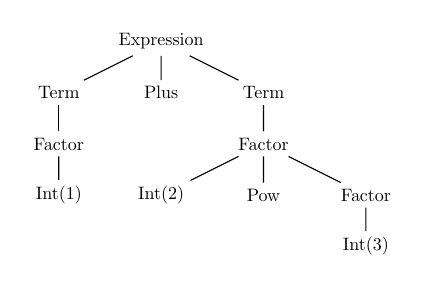
\begin{tikzpicture}[level distance=1cm, sibling distance=2cm, scale=.65, transform shape]
				\node {Expression}
				child {node {Term}
						child {node {Factor}
								child {node {\Verb{Int(1)}}}}}
				child {node {\Verb{Plus}}}
				child {node {Term}
						child {node {Factor}
								child {node {\Verb{Int(2)}}}
								child {node {\Verb{Pow}}}
								child {node {Factor}
										child {node {\Verb{Int(3)}}}}}};
			\end{tikzpicture}
			\caption{Abstakter Syntaxbaum für `\texttt{1+2**3}'.}\label{fig:parser_simple_ast}
		\end{minipage}
        \hfill
		\begin{minipage}{.45\textwidth}
			\begin{figure}[h]
				\centering
				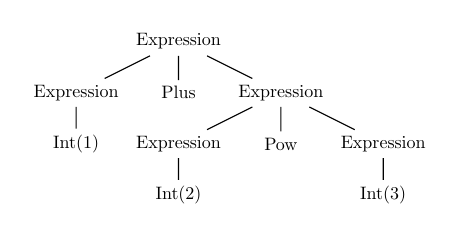
\begin{tikzpicture}[level distance=1cm, sibling distance=2cm, scale=.65, transform shape]
					\node {Expression}
					child {node {Expression}
							child {node {\Verb{Int(1)}}}}
					child {node {\Verb{Plus}}}
					child {node {Expression}
							child {node {Expression}
									child {node {\Verb{Int(2)}}}}
							child {node {\Verb{Pow}}}
							child {node {Expression}
									child {node {\Verb{Int(3)}}}}};
				\end{tikzpicture}
				\caption{Abstakter Syntaxbaum für `\texttt{1+2**3}', erstellt durch Pratt-Parsing.}\label{fig:parser_simple_ast_pratt}
			\end{figure}
		\end{minipage}
	\end{figure}
\end{frame}
